% DO NOT COMPILE THIS FILE DIRECTLY!
% This is included by the other .tex files.

\begin{frame}[t,plain]
\titlepage
\end{frame}

\begin{frame}{Agenda}
    \input{../includes/agenda.txt}
\end{frame}

\begin{frame}
 \frametitle{MISP, bekeken vanuit een praktisch voorbeeld}
 \begin{itemize}
         \item In 2012 werd tijdens een werkgroep voor malware analyse duidelijk dat we werkten aan de analyse van dezelfde malware.
         \item We wilden onze informatie op een eenvoudige en geautomatiseerde manier met elkaar delen {\bf om dubbel werk te voorkomen}.
         \item Christophe Vandeplas (toen werkzaam bij het CERT voor de Belgische Defensie) toonde ons zijn werk aan een platform dat uiteindelijk MISP werd.
         \item De eerste versie van het MISP-platform werd gebruikt door de MALWG en met hulp van {\bf de toenemende feedback van gebruikers} konden we een verbeterd platform bouwen.
         \item MISP is nu uitgegroeid tot een platform waar de {\bf ontwikkeling gestuurd wordt vanuit de gemeenschap}.
 \end{itemize}
\end{frame}

\begin{frame}
\frametitle{over CIRCL}
Het Computer Incident Response Centre Luxembourg (CIRCL) is een overheids initiatief om een antwoord te bieden op computerbeveiligingsbedreigingen en -incidenten. \break \newline
CIRCL is het CERT voor de particuliere sector, gemeenten en niet-gouvernementele entiteiten in Luxemburg en wordt beheerd door securitymadein.lu g.i.e.
\end{frame}

\begin{frame}
\frametitle{MISP en CIRCL}
\begin{itemize}
\item CIRCL is gemandateerd door het ministerie van Economische Zaken en treedt op als het Luxemburgse nationale CERT voor de particuliere sector.
\item CIRCL leidt de ontwikkeling van het Open Source MISP-platform voor het delen van dreigingsinformatie. Dit platform is wereldwijd gebruikt door veel militaire en inlichtingengemeenschappen, privébedrijven, de financiële sector, nationale CERT's en LEA's.
\item {\bf CIRCL beheert meerdere grote MISP-gemeenschappen die dagelijkse actief zijn in het delen van dreigingsinformatie}.
\end{itemize}
        \includegraphics{en_cef.png}
\end{frame}


\begin{frame}
\frametitle{Ontwikkeling gebaseerd op praktische feedback van de gebruikers}
\begin{itemize}
\item Er zijn veel verschillende soorten gebruikers van een informatie-uitwisselingsplatform zoals MISP:
        \begin{itemize}
                \item {\bf Malware-analysten} die bereid zijn om de indicatoren van hun analyse met collega's te delen.
                \item {\bf Beveiligingsanalisten} die voor operationele beveiliging zoeken naar indicatoren, deze valideren en gebruiken.
                \item {\bf Informatie-analysten} die informatie verzamelen over specifieke vijandige groepen.
                \item De {\bf politie} die vertrouwt op indicatoren om digitale onderzoeken te ondersteunen of op te starten.
                \item {\bf Risico analyse teams} die meer willen weten over nieuwe dreigingen, de waarschijnlijkheid van deze dreigingen en of deze dreigingen werden vastgesteld.
                \item {\bf Fraude analysten} die bereid zijn om indicatoren te delen om financiële fraude op te sporen.
        \end{itemize}
\end{itemize}
\end{frame}

\begin{frame}
\frametitle{Het beheermodel van MISP}
\includegraphics[scale=0.4]{governance.png}
\end{frame}

\begin{frame}
\frametitle{Verschillende objectieven}
        \begin{itemize}
                \item Delen van indicatoren voor {\bf detectie} doeleinden.
                        \begin{itemize}
                                \item 'Heb ik geïnfecteerde systemen in mijn infrastructuur of onder mijn beheer?'
                        \end{itemize}
                \item Delen van  indicatoren om te {\bf blokkeren}.
                        \begin{itemize}
                                \item 'Ik gebruik deze attributen om verkeer te blokkeren of om verkeer om te leiden.'
                        \end{itemize}
                \item Delen van  indicatoren om {\bf informatie te verzamelen}.
                        \begin{itemize}
                                \item 'Informatie verzamelen over campagnes en aanvallen. Zijn deze campagnes met elkaar verbonden? Zijn ze gericht op mij? Wie zijn de tegenstanders?'
                        \end{itemize}
                \item $\rightarrow$ Deze doelstellingen kunnen soms tegenstrijdig zijn
        \end{itemize}
\end{frame}

\begin{frame}
\frametitle{Moeilijkheden bij het delen}
        \begin{itemize}
                \item De problemen met het delen van informatie zijn vaak niet zozeer van technische aard maar eerder een kwestie van {\bf sociale interacties} (b.v. {\bf vertrouwen}).
                \item Juridische restricties\footnote{\url{https://www.misp-project.org/compliance/}}
                        \begin{itemize}
                                \item "Ons wettelijk kader staat ons niet toe om informatie te delen."
                                \item "Het risico op een informatielek is te hoog en het is te riskant voor onze organisatie of partners."
                        \end{itemize}
                \item Praktische beperkingen
                        \begin{itemize}
                                \item "We hebben geen informatie om te delen."
                                \item "We hebben geen tijd om indicatoren te verwerken of om er te delen."
                                \item "Ons classificatie model past niet in uw model."
                                \item "De middelen voor het delen van informatie zijn gebonden aan een specifiek formaat en we gebruiken een ander formaat."
                        \end{itemize}
        \end{itemize}
\end{frame}


\begin{frame}
        \frametitle{MISP Project Overzicht}
        \includegraphics[scale=0.35]{misp-overview-simplified.pdf}
\end{frame}

%\begin{frame}
%        \frametitle{MISP Project Overview}
%        \begin{columns}[t]
%        \column{5.0cm}
%        \begin{figure}
%        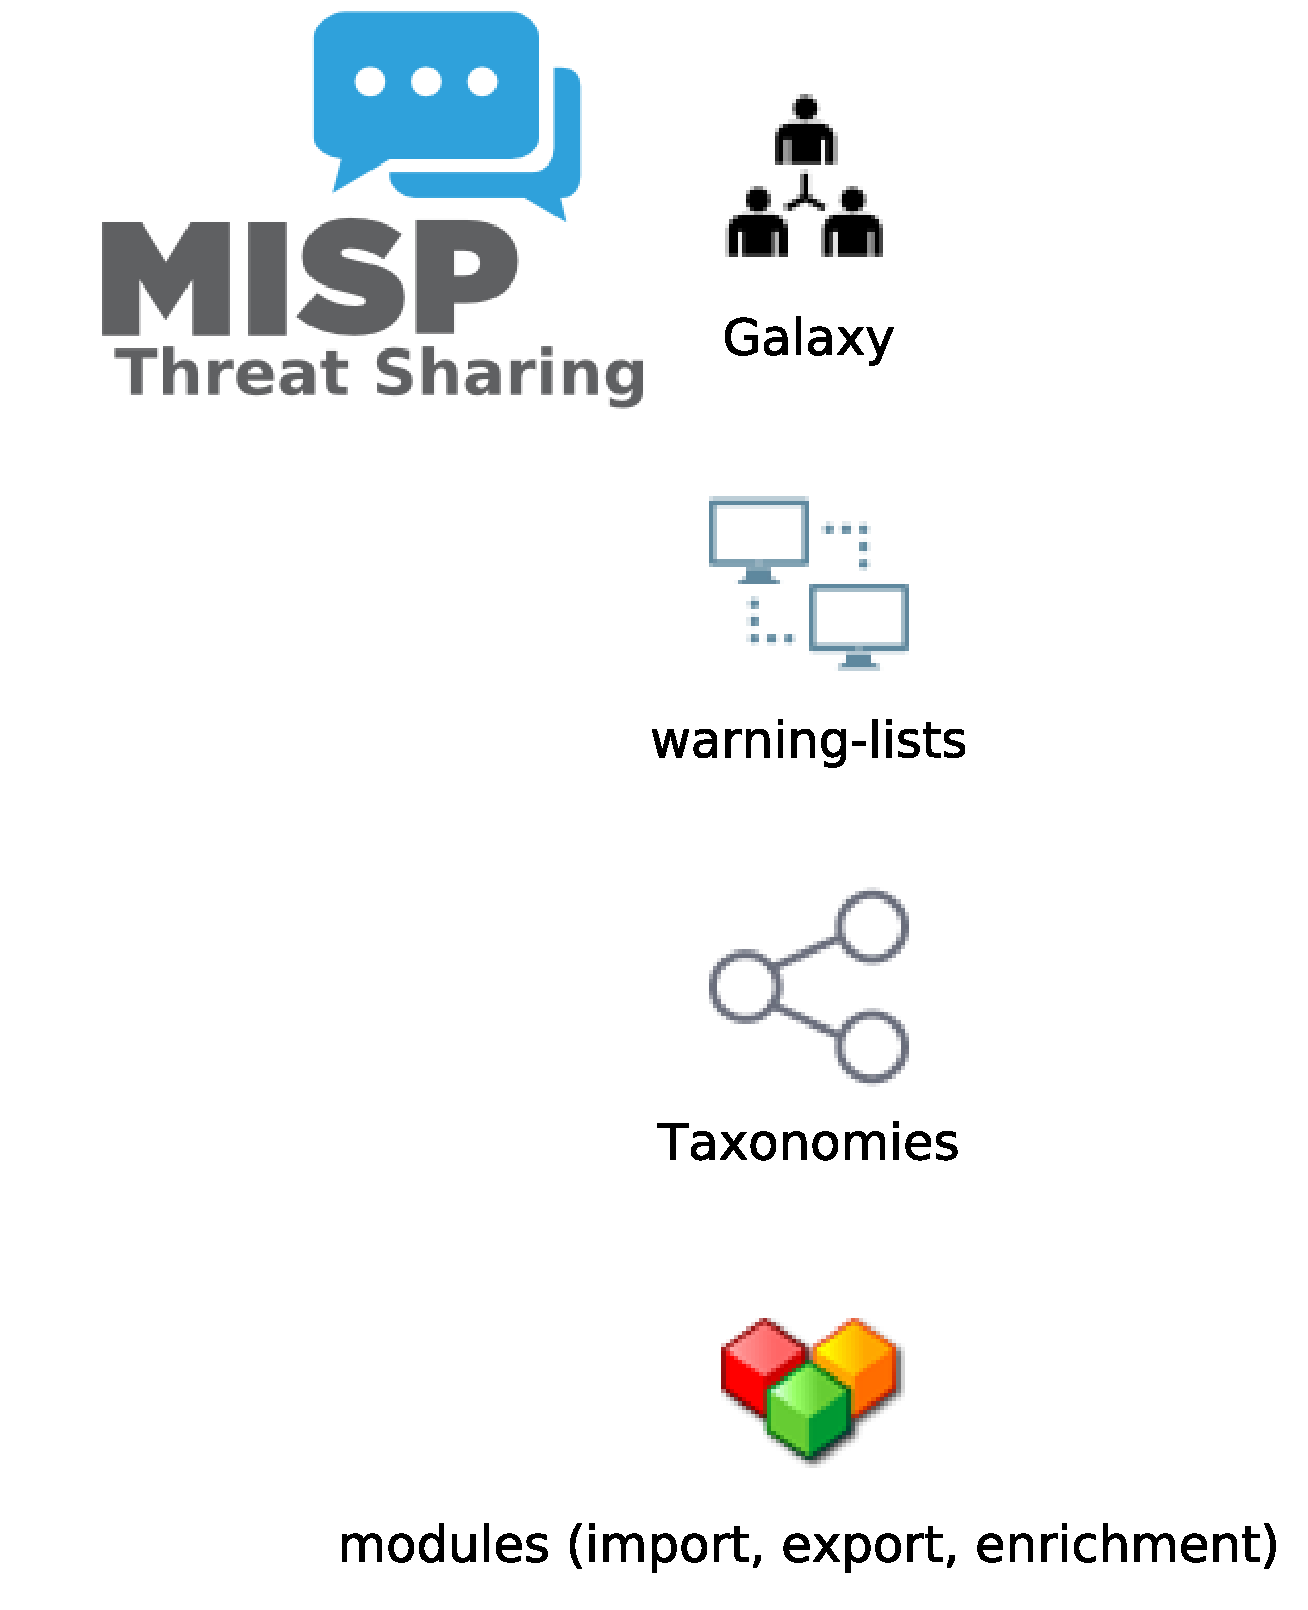
\includegraphics[scale=0.20]{misp-overview.pdf}\\
%        \end{figure}
%        \column{7cm}
%        \begin{itemize}
%                \item The {\bf core project}\footnote{\url{http://github.com/MISP/}} (PHP/Python3) supports the backend, API \& UI.
%                \item Modules (Python3) expand MISP functionalities.
%                \item Taxonomies (JSON) to add categories \& global tagging.
%                \item Warning-lists (JSON) help analysts to detect potential false-positives.
%                \item Galaxy (JSON) to add threat-actors, tools or "intelligence".
%                \item Objects (JSON) to allow for templated composition of security related atomic points of information.
%        \end{itemize}
%        \end{columns}
%\end{frame}

\begin{frame}
 \frametitle{MISP functies}
 \begin{itemize}
         \item MISP\footnote{\url{https://github.com/MISP/MISP}} is open source software voor het delen van dreigings-informatie.
         \item MISP heeft {\bf een groot aantal functionaliteiten} die gebruikers ondersteunen bij het maken, samen werken aan en het delen van bedreigingsinformatie - bijv. flexibele groepen voor het delen van informatie, {\bf automatische correlatie van gegevens}, importhulp, event distributie en voorstelling voor verbetering van attributen.
         \item Er is ondersteuning voor diverse formaten van IDS / IPS systemen (b.v. Suricata, Bro, Snort), SIEMs (b.v. CEF), host scanners (b.v. OpenIOC, STIX, CSV, yara), analyse tools (b.v. Maltego) of om DNS policies te implementeren (b.v. RPZ).
         \item Er is een breed aanbod aan MISP modules\footnote{\url{https://www.github.com/MISP/misp-modules}} voor uitbreiding, import en export functionaliteiten.
 \end{itemize}
\end{frame}

\begin{frame}
        \frametitle{Correlaties : een hulpmiddel voor analysten}
        \includegraphics[scale=0.18]{screenshots/campaign.png}
        \begin{itemize}
                \item Voor het {\bf  bevestigen van een bevinding} (b.v. is dit dezelfde campagne?), {\bf of een analyse} (b.v. hebben andere analysten dezelfde hypothesis?), {\bf bevestigen van een specifiek aspect} (b.v. werden deze sinkhole IP adressen gebruikt voor een campagne?) of het simpelweg uitzoeken of een {\bf dreiging nieuw of onbekend is in je omgeving}.
        \end{itemize}
\end{frame}


\begin{frame}
 \frametitle{Groepen die MISP gebruiken}
 \begin{itemize}
	 \item In het algemeen gaan gebruikers informatie delen met een groep met dezelfde objectieven of waarden.
	 \item CIRCL beheert meerdere MISP-instanties met een aanzienlijke gebruikersbasis (meer dan 950 organisaties met meer dan 2400 gebruikers).
     \item {\bf Vertrouwde} (gesloten) groepen die MISP gebruiken in een soort "eiland" modus (als een geïsoleerd systeem) of als een deels geconnecteerd systeem.
	 \item De {\bf financiële sector} (banken, ISACs, organisaties die betalingen verwerken) gebruikt MISP als een mechanisme voor het delen van informatie.
	 \item {\bf Militaire en internationale organisaties} (NATO, militaire CSIRTs, n/g CERTs,...).
	 \item {\bf Security bedrijven} die hun eigen gemeenschap starten (b.v. Fidelis) of een koppeling hebben met een MISP gemeenschap (b.v. OTX).
 \end{itemize}
\end{frame}


\begin{frame}
\frametitle{MISP basisfuncties voor gedistribueerd delen}
\begin{itemize}
\item De kernfunctionaliteit van MISP is het delen van informatie waarbij iedereen zowel een consument als een producent (bijdrager) kan zijn.
\item Dit heeft als voordeel dat iedereen snel kan deelnemen, zonder de directe verplichting om zelf bij te dragen.
\item Er is een lage drempel om het systeem te leren kennen.
\end{itemize}
\includegraphics[scale=0.9]{misp-distributed.pdf}
\end{frame}


\begin{frame}
        \frametitle{Events, Objecten en Attributen in MISP}
         \begin{itemize}
                \item Een MISP event is een verzameling van contextueel verbonden informatie.
                \item Attributen\footnote{attributen kunnen alles zijn zolang ze bijdragen aan het beschrijven van de intentie van het event, b.v. indicatoren, kwetsbaarheden ... } starten initieel met een standaard groep van "cyber security" indicatoren.
                \item Attributen zijn puur {\bf gebaseerd op gebruik}. De verbetering gebeuren voornamelijk op basis van praktische noden ({\bf financiële indicatoren} in versie 2.4).
                \item Objecten zijn samengestelde attributen die verschillende datapunten beschrijven, opgebouwd uit templates van de gemeenschap en de gebruikers.
                \item Galaxies zorgen voor een granulaire context, classificatie en categorisatie van de gegevens gebaseerd op {\bf dreigings actoren}, {\bf preventie  maatregelen} en de hulpmiddelen gebruikt door tegenstanders.
        \end{itemize}
\end{frame}

\begin{frame}
        \frametitle{Delen van Technieken van Aanvallers}
        \begin{itemize}
                \item MISP heeft integratie op zowel event als attribuut niveau voor MITRE's Adversarial Tactics, Techniques, and Common Knowledge (ATT\&CK).
        \end{itemize}
        \includegraphics[scale=0.2]{screenshots/attack-screenshot.png}
\end{frame}

\begin{frame}
        \frametitle{Ondersteuning voor een specifiek datamodel}
        \includegraphics[scale=0.24]{screenshots/bankaccount.png}
        \includegraphics[scale=0.18]{screenshots/bankview.png}
\end{frame}

\begin{frame}
        \frametitle{Terminilogie van indicatoren}
        \begin{itemize}
                \item Indicatoren\footnote{IoC (Indicator of Compromise) zijn een onderdeel van de indicatoren}
                        \begin{itemize}
                                \item Indicatoren beschrijven een patroon dat kan gebruikt worden om verdachte of kwaadaardige traffiek te detecteren.
                        \end{itemize}
                \item Attributen in MISP kunnen netwerk indicatoren (b.v. IP adressen), systeem indicatoren (b.v. tekst in het geheugen) of zelfs bank gegevens zijn.
                \begin{itemize}
                        \item Een {\bf type} (b.v. MD5, url) is hoe een attribuut is beschreven.
                \end{itemize}
                \begin{itemize}
                \item Een attribuut behoort altijd tot een categorie (b.v. Payload delivery). Deze categorie plaatst het attribuut in een bepaalde context.
                        \begin{itemize}
                                \item {\bf Een categorie bepaalt de context } van een attribuut.
                        \end{itemize}
                \item De IDS instelling op een attribuut bepaald of {\bf dit attribuut automatisch} zal gebruikt worden voor {\bf detectie} doeleinden.
                \end{itemize}
        \end{itemize}
\end{frame}

\begin{frame}
        \frametitle{Ondersteuning voor het werken met MISP}
        \begin{itemize}
            \item Gebruikers kunnen events of attributen bijvoegen via zowel de web interface, de API als via een vrije tekst veld.
                \begin{itemize}
                        \item Er zijn modules in Viper (een framework voor het analyseren van malware) om data in MISP in te vullen, via de vty of via IDA.
                \end{itemize}
        \item Een bijdrage kan gebeuren door rechtstreeks een event aan te maken maar gebruikers kunnen ook de eigenaar van een event een {\bf update voorstellen voor attributen}.
            \item Gebruikers zijn {\bf niet gedwongen om één interface te gebruiken om gegevens aan MISP bij te voegen}.
        \end{itemize}
\end{frame}

\begin{frame}
        \frametitle{Voorbeeld: Vrije tekst import in MISP}
        \includegraphics[scale=0.3]{screenshots/freetext1.PNG}\\
        \includegraphics[scale=0.3]{screenshots/freetxt2.PNG}\\
        \includegraphics[scale=0.3]{screenshots/freetxt3.PNG}
\end{frame}

\begin{frame}
        \frametitle{Ondersteuning voor classificaties}
        \begin{itemize}
          \item Het gebruik van tags is een simpele manier om een classificatie toe te voegen aan een event of attribuut.
          \item Een {\bf classificatie moet globaal} in gebruik zijn om ook efficient te zijn.
          \item Gebruikers kunnen via een flexibel tagging systeem kiezen uit de meer dan 42 bestaande taxonomieën of ze kunnen hun eigen taxonomie bijvoegen.
        \end{itemize}
        \includegraphics[scale=0.20]{tags-2-4-70.png}
\end{frame}

\begin{frame}
\frametitle{Ondersteuning voor het delen in MISP}
\begin{itemize}
        \item Delegeren van de publicatie van events naar andere organisaties (sinds MISP 2.4.18).
        \begin{itemize}
                \item Deze andere organisatie kan dan eigenaar worden van het event en op deze manier zorgen voor de {\bf pseudo-anonimiteit van de oorspronkelijke organisatie}.
        \end{itemize}
        \item Definiëren van groepen om specifieke informatie mee te delen (vanaf 2.4).
        \begin{itemize}
                \item De gemeenschappen om mee te delen kunnen lokaal of tussen verschillende MISP instanties gebruikt worden.
                \item Het delen kan gebeuren op zowel {\bf event} als {\bf attribuut} niveau (b.v. financiële indicatoren met de financiële groepen en cyber security indicatoren met de CSIRT gemeenschap).
        \end{itemize}
\end{itemize}
\end{frame}

\begin{frame}
        \frametitle{Ondersteuning voor waarnemingen}
        \begin{columns}[t]
        \column{5.0cm}
        \begin{figure}
        \includegraphics[scale=0.3]{screenshots/sighting-n.png}\\
        \includegraphics[scale=0.34]{screenshots/Sightings2.PNG}
        \end{figure}
        \column{7cm}
        \begin{itemize}
                \item Gebruikers kunnen via {\bf waarnemingen} de gemeenschap op de hoogte stellen van activiteit gerelateerd aan een indicator.
                \item Het is mogelijk om negatieve waarnemingen (false positives) en waarnemingen met een vervaldatum in te geven.
                \item Waarnemingen kunnen gebeuren via de web interface, de API of door STIX waarnemings-documenten te importeren.
                \item Er zijn verschillende toepassingen om indicatoren te rangschikken op basis van waarnemingen.
        \end{itemize}
        \end{columns}
\end{frame}


\begin{frame}
\frametitle{Verbeteringen voor het delen van informatie in MISP}
\begin{itemize}
        \item Valse positiven (false-positive) blijven een terugkerende uitdaging bij het delen van informatie.
        \item Vanaf MISP 2.4.39 hebben we het concept van misp-warninglists\footnote{\url{https://github.com/MISP/misp-warninglists}} geïntroduceerd om de analysten te ondersteunen bij hun dagtaak.
        \item Dit zijn voorgedefinieerde lijsten van indicatoren die vaak een valse positieve zijn, zoals bijvoorbeeld RFC1918 netwerken of publieke DNS servers.
\end{itemize}
\end{frame}

\begin{frame}
\frametitle{Ondersteuninng voor het delen binnen en buiten een organisatie}
\begin{itemize}
        \item Zelfs binnen één en dezelfde omgeving kunnen er verschillende use cases zijn voor het gebruik van MISP (b.v. groepen die MISP gebruiken voor dynamische malware analyse en correlatie, andere groepen die het dan weer gebruiken voor het versturen van meldingen).
        \item Vanaf MISP 2.4.51, is er de optie om {\bf lokale MISP} servers met elkaar te verbinden. Zo kan je verschillende niveaus van delen voorkomen en kan je van een gemengde synchronisatie gebruik maken, zowel binnen als buiten de organisatie.
        \item Er is ondersteuning voor feeds voor synchronisatie tussen vertrouwde en niet vertrouwde netwerken.
\end{itemize}
\end{frame}

\begin{frame}
        \frametitle{Starten met MISP en indicatoren}
        \begin{itemize}
                \item We onderhouden de standaard CIRCL OSINT-feeds (TLP:WHITE geselecteerd uit onze gemeenschappen) zodat gebruikers snel aan de slag kunnen gaan met MISP.
                \item Het formaat van de OSINT-feed is gebaseerd op standaard MISP JSON-uitvoer van een externe TLS / HTTP-server.
                \item Aanvullende contentproviders kunnen hun eigen MISP-feeds leveren. (\url{https://botvrij.eu/}).
                \item Dit laat gebruikers toe om hun MISP-installaties te {\bf testen en te synchroniseren met een echte gegevensset}.
                \item Dit kan bijdragen aan andere bronnen van dreigings informatie en helpt ook bij de analyze naar overlappende data\footnote{Een steeds terugkerende uitdaging bij het delen van informatie}.
        \end{itemize}
\end{frame}


\begin{frame}
        \frametitle{Conclusie}
        \begin{itemize}
                \item {\bf De manier van informatie delen onstaat voornamelijk uit het gebruik} en het volgen van bestaande voorbeelden.
                \item MISP is uiteindelijk slechts een hulpmiddel, het belangrijkste is nog altijd de manier hoe je de informatie deelt. De tool moet u daarbij zo transparant mogelijk ondersteunen tijdens uw werk.
                \item Gebruikers moeten MISP kunnen aanpassen zodat zij een oplossing hebben voor de noden van hun gemeenschap.
                \item Het MISP project combineert open source software, open standaarden, best practices en gemeenschappen om informatie deling te realiseren.
        \end{itemize}
\end{frame}

